\section{GPU Programming}
CUDA für Nvidia Karten und OpenCL für HW-Unabhängig Programmierung von GPU.

\subsection{Performance}
Siehe auch Kapitel \ref{performance}.
\begin{center}
	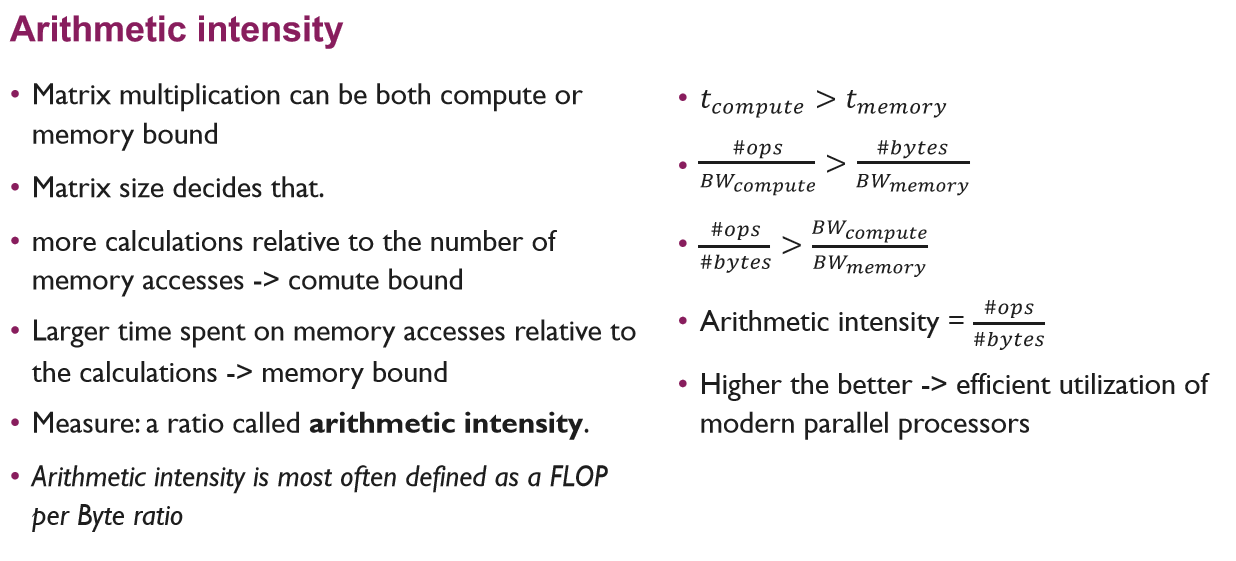
\includegraphics[width=\columnwidth]{Images/intensity}
\end{center}


\subsection{CUDA Execution Model}
CUDA ist in Blocks (auch Streaming Multiprocessor) aufgeteilt, welche wiederum aus \textit{Threads} (auch Streaming Processor) besteht. Jeder Thread hat eine eigene Id (x, y und z), um auf Daten zuzugreifen.

\begin{center}
	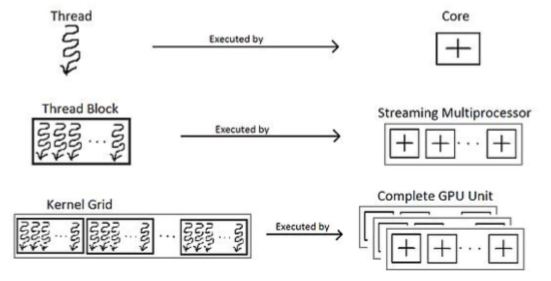
\includegraphics[width=0.9\columnwidth]{Images/gpu}
\end{center}

\begin{lstlisting}
// kernel definition for CUDA, executed on GPU
__global__ void parallelSum(int* array, int length) {
	int offset = blockIdx.x * blockDim.x;
	int stride = 1;
	while (stride < blockDim.x) {
		int first = offset + 2 * stride * threadIdx.x;
		int second = first + stride;
		if (second < length) {
			array[first] += array[second];
		}
		stride *= 2;
		__syncthreads();
	}
}

__global__ void matrixMultiply(float *A, float *B, float *C) {
	int col = blockIdx.x * blockDim.x + threadIdx.x;
	int row = blockIdx.y * blockDim.y + threadIdx.y;
	float sum = 0.0f;
	
	if (row < C_ROWS && col < C_COLS) {
		for (int k = 0; k < A_COLS; k++) {
			sum += A[row * A_COLS + k] * B[k * B_COLS + col];
		}
		
		C[row * C_COLS + col] = sum;
	}
}

// executet on CPU (Host)
int main() {
	// (1) alloc GPU memory
	cudaMalloc(..); 		
	// (2) transfer Data to GPU			
	cudaMemcpy(dst, src, size, dir); 
	// (3) kernel invocation	
	parallelSum<<<1, N>>>(A,B); 
	
    dim3 threadsPerBlock(tile_size, tile_size);
	dim3 blocksPerGrid((C_COLS + tile_size - 1) / tile_size, (C_ROWS + tile_size - 1) / tile_size);
	
	matrixMultiply<<<blocksPerGrid, threadsPerBlock>>>(d_a, d_b, d_c);
	
	// (4) transfer Data to CPU	
	cudaMemcpy(dst, src, size, dir); 
	// (5) free data	
	cudaFree(..);						
}
\end{lstlisting}

\subsection{Cuda Grid}
\textbf{threadIdx.x} greift auf Thread number im Block zu, \textbf{blockIdx.x} beinhaltet die Block Nummer und \textbf{blockDim.x} die Block grösse.
\begin{center}
\begin{lstlisting}
	int N = 32;
	dim3 grid = (8,4,2); // x, y, z => 64 blocks
	dim3 block = (N, 1, 1); // x, y, z => 32 threads per block
	VectorAddKernel<<<grid, block>>>(A,B,C);
	
	int threadsPerBlock = 256;
	int blocksPerGrid = (N + threadsPerBlock - 1) / threadsPerBlock;
	VectorAddKernel<<<blocksPerGrid, threadsPerBlock>>>(A,B,C);
\end{lstlisting}
	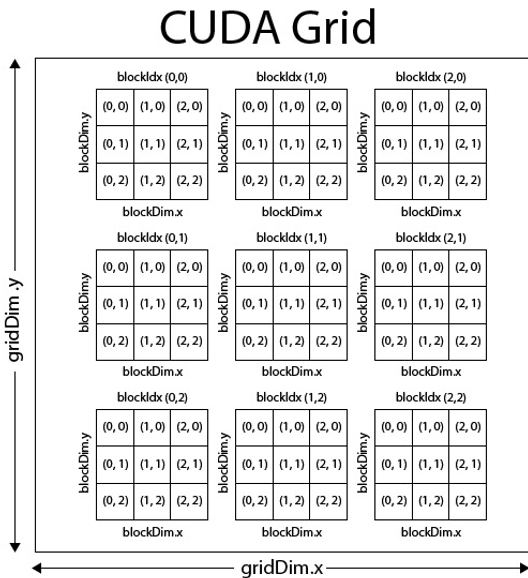
\includegraphics[width=0.6\columnwidth]{Images/grid}
\end{center}
Um auf die Daten in Array zuzugreifen kann pro Thread folgende Formel verwendet werden:
\[
index = blockIdx.x * blockDim.x + threadIdx.x
\]

\subsection{Performance}
\subsection{Divergence, Warp Exceution}
Alle Threads auf GPU sollten gleiche Instruktionen ausführen, sonst müssen diese aufeinander Warten und sind dadurch blockiert. Problem bei if/for/do/switch statements, weil diese Unterschiedliche Laufzeiten aufweisen können. Daher pro Warp gleiche Ausführung forcieren:
\begin{lstlisting}
if (threadIdx.x > 1) { } // BAD
if (threadIdx.x / 32 > 1) { } // GOOD
\end{lstlisting}

\subsection{Coalesing}
Pro Warp sollten auf gleiche Daten zugegriffen werden, um Performance zu erhöhen. Dies wird Coalescing genannt. Ein Zwischenfall ist Strided Coalescing.
\begin{center}
	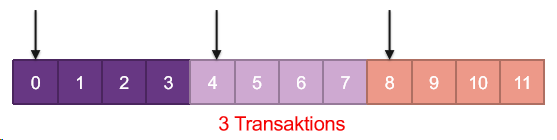
\includegraphics[width=0.8\columnwidth]{Sections/coalescing}
\end{center}
